\subsection{Simpler models: only the bias and the lapses need to vary between sessions}\label{sec:simpler}
Model~D lets eight parameters per hand vary from session to session. The simpler versions hold some of them fixed (Fig.~\ref{fig:complexity}, Table~\ref{tab:comparison}).
\begin{itemize}
\item \textbf{The bias must vary.} With no session differences at all, D0 minus D is \DzerovsDTrial\ at the trial level.
\item \textbf{The distractor terms need not vary.} Holding $b_2$ and $b_3$ fixed for each hand (D4 minus D: \DfourvsDTrial\ $\pm$ \DfourvsDTrialSE\ at the trial level, \DfourvsDLoso\ $\pm$ \DfourvsDLosoSE\ for new sessions) saves 4 parameters per session and 20 effective parameters (\plooD\ $\to$ \plooDfour). Once its amplitude is taken into account, the distractor has the same effect in every session.
\item \textbf{Neither, largely, does the slope.} Holding it fixed as well changes little (D3 minus D2: \DthreevsDtwoTrial\ $\pm$ \DthreevsDtwoTrialSE\ at the trial level, \DthreevsDtwoLoso\ $\pm$ \DthreevsDtwoLosoSE\ for new sessions).
\item \textbf{The lapse rates do vary.} Holding them fixed loses ground (D1 minus D: \DonevsDTrial\ $\pm$ \DonevsDTrialSE\ at the trial level, \DonevsDLoso\ $\pm$ \DonevsDLosoSE\ for new sessions), and this step accounts for most of what the simpler models D2 and D3 lose.
\end{itemize}

The same simplifications hold with the criterion trend.
\textbf{Model~E} (D4+crit: bias, slope and lapses vary between sessions, the distractor terms are fixed per hand, and the bias follows the distractor amplitude) is as good as D+crit (E minus D+crit: \DfourCritvsCritTrial\ $\pm$ \DfourCritvsCritTrialSE\ at the trial level, \DfourCritvsCritLoso\ $\pm$ \DfourCritvsCritLosoSE\ for new sessions) with 20 fewer effective parameters (\plooDfourCrit\ against \plooCrit).
It beats D by \DfourCritvsDLoso\ $\pm$ \DfourCritvsDLosoSE\ and B by \DfourCritvsBLoso\ $\pm$ \DfourCritvsBLosoSE\ for new sessions.
Even D3+crit, with a single bias per hand and session (2 parameters per session against 16 in B and D), predicts new sessions as well as D (\DthreeCritvsDLoso\ $\pm$ \DthreeCritvsDLosoSE) and better than B (\DthreeCritvsBLoso\ $\pm$ \DthreeCritvsBLosoSE), with fewer than half of B's effective parameters (\plooDthreeCrit\ against \plooB).

\begin{figure}[tbp]
\centering
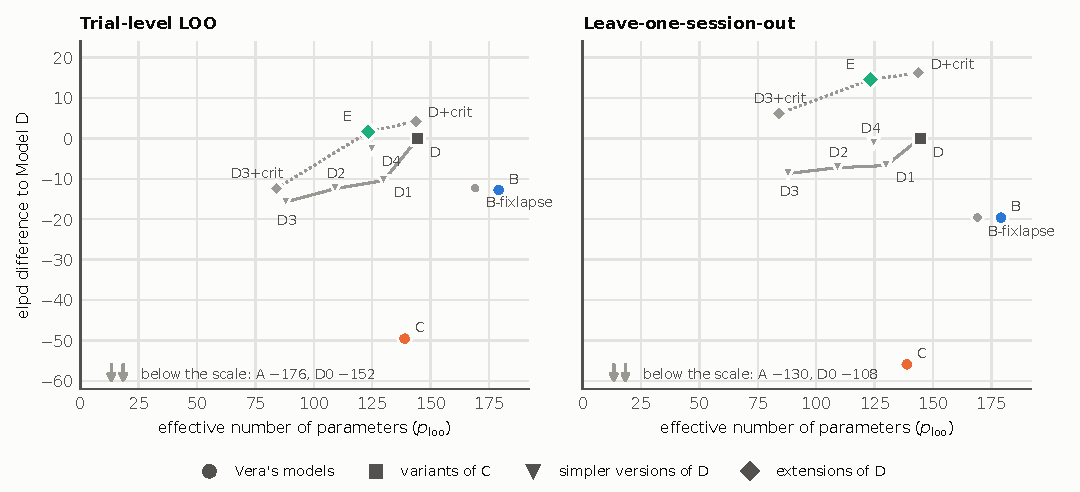
\includegraphics[width=\textwidth]{../results5000/figs/F2_complexity.pdf}
\caption{Predictive performance against model complexity (effective number of parameters, $p_\mathrm{loo}$), relative to Model~D (dashed line).
Solid grey line: the simpler versions of D, from D3 (only the bias varies between sessions) through D2 and D1 to D.
Dotted grey line: the same with the criterion trend, from D3+crit through E to D+crit.}\label{fig:complexity}
\end{figure}
